\begin{figure}[htbp]
    \centering
    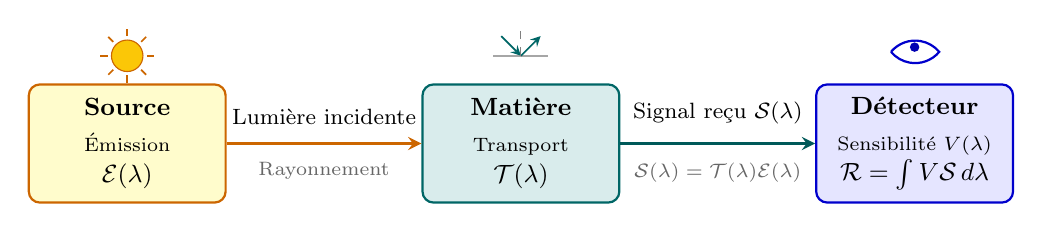
\begin{tikzpicture}[
        node distance=5cm,
        block/.style={
            draw, 
            rounded corners=4pt, 
            line width=0.8pt, 
            minimum width=2.5cm, 
            minimum height=1.5cm, 
            align=center, 
            font=\small
        },
        ray/.style={
            ->, 
            >=stealth, 
            very thick, 
            line width=1.1pt
        }
    ]
        % --- 1. Source de lumière ---
        \node[block, fill=yellow!20, draw=orange!80!black] (source) {
            \textbf{Source}\\[2pt]
            \scriptsize Émission\\
            $\mathcal{E}(\lambda)$
        };

        % --- 2. Objet / Interaction avec la matière ---
        \node[block, fill=teal!15, draw=teal!80!black, right of=source] (object) {
            \textbf{Matière}\\[2pt]
            \scriptsize Transport\\
            $\mathcal{T}(\lambda)$
        };

        % --- 3. Détecteur / Capteur (Œil / Caméra) ---
        \node[block, fill=blue!10, draw=blue!80!black, right of=object] (sensor) {
            \textbf{Détecteur}\\[2pt]
            \scriptsize Sensibilité $V(\lambda)$\\
            $\mathcal{R} = \int V\mathcal{S}\,d\lambda$
        };

        % --- Rayons lumineux et annotations aérées ---
        % Rayon incident
        \draw[ray, orange!80!black] (source) -- (object) 
            node[midway, above=3pt, font=\footnotesize, text=black] {Lumière incidente}
            node[midway, below=3pt, font=\scriptsize, text=gray!80!black] {Rayonnement};

        % Rayon réfléchi / transporté
        \draw[ray, teal!70!black] (object) -- (sensor) 
            node[midway, above=3pt, font=\footnotesize, text=black] {Signal reçu $\mathcal{S}(\lambda)$}
            node[midway, below=3pt, font=\scriptsize, text=gray!80!black] {$\mathcal{S}(\lambda) = \mathcal{T}(\lambda)\mathcal{E}(\lambda)$};

        % --- Icônes minimalistes géométriques ---
        % Soleil schématisé
        \begin{scope}[shift={(source.north)}, yshift=0.35cm]
            \draw[fill=yellow!60!orange, draw=orange!80!black] (0,0) circle (0.2cm);
            \foreach \a in {0, 45, 90, 135, 180, 225, 270, 315} {
                \draw[orange!80!black, semithick] (\a:0.25cm) -- (\a:0.34cm);
            }
        \end{scope}

        % Symbole de réflexion surfacique
        \begin{scope}[shift={(object.north)}, yshift=0.35cm]
            \draw[thick, gray!70] (-0.35, 0) -- (0.35, 0);
            \draw[->, >=stealth, semithick, teal!80!black] (-0.25, 0.25) -- (0, 0);
            \draw[->, >=stealth, semithick, teal!80!black] (0, 0) -- (0.25, 0.25);
            \draw[thin, dashed, gray] (0, 0) -- (0, 0.35);
        \end{scope}

        % Symbole de capteur / œil
        \begin{scope}[shift={(sensor.north)}, yshift=0.4cm]
            \draw[thick, blue!80!black] (-0.3, 0) arc (140:40:0.4) arc (-40:-140:0.4);
            \fill[blue!70!black] (0, 0.06) circle (0.06);
        \end{scope}
    \end{tikzpicture}
    \caption{Chaîne fondamentale de formation de l'image en synthèse d'images : de l'émission à la réponse du capteur.}
    \label{fig:chaine_rendu_principe}
\end{figure}